\documentclass{article}

% Includes preamble from standard file
% ==========================================================
%   GPR-20 MANUALS PREAMBLE
% ==========================================================

% ==========================================================
% Includes packages
\usepackage{array}
\usepackage{float}
\usepackage{amssymb}
\usepackage{amsmath}
\usepackage{parskip}
\usepackage{caption}
\usepackage{tabularx}
\usepackage{titlesec}
\usepackage{hyperref}
\usepackage{setspace}
\usepackage{graphicx}
\usepackage{listings}
\usepackage{csvsimple}
\usepackage{longtable}
\usepackage{xltabular}
\usepackage{subcaption}
\usepackage{indentfirst}
\usepackage[utf8]{inputenc}
\usepackage[margin=1in]{geometry}
\usepackage[type={CC}, modifier={by-nc}, version={4.0}]{doclicense}
\usepackage{subfiles}
% ==========================================================

% ==========================================================
% PREAMBLE SETTINGS
% Sets double spacing
\doublespacing

% Sets paragraph indentation
\setlength{\parindent}{1em}

% Sets paragraph skip
\setlength{\parskip}{2em}

% Starts section on new page
\newcommand{\sectionbreak}{\clearpage}

\renewcommand{\arraystretch}{1.25}
% ==========================================================


% Adds bibliography
\usepackage[style=numeric]{biblatex}
\bibliography{biblio.bib}


% Defines command to insert name
\newcommand{\GPRManualName}{Data Acquisition Guide}

% ==========================================================
% DOCUMENT INFORMATION
\title{GPR-20: Data Acquisition Guide}
\author{Grupo de Desminado Humanitario}
\date{January 2022}
% ==========================================================

\begin{document}

\subfile{front}

\section{Introduction}
The GPR-20 robot is a data-acquisition instrument that aims to improve the understanding of demining operations. The robot consists of an implementation of the Ground Penetrating Radar (GPR) technique to acquire data that allows to scan the soil. The GPR uses electromagnetic waves to scan the subsurface and to provide an insight of the elements that are located underground. The GPR relies on the reflection of electromagnetic waves to identify boundaries between elements of the ground e.g. where the type of soil or where an object, such as a landmine, is buried. Applications in the fields of archaeology, Earth sciences and social sciences can also benefit from the GPR technique.

The GPR is implemented in the robot by the means of a Vector Network Analyzer (VNA) and two antennae. The group of the VNA and the antennae is defined as the GPR within the context of the robot. The GPR allows to acquire the scattering parameters of the soil. Each sample is located in a fixed physical location that can be identified with a pair of coordinates. By sampling multiple coordinates within a sampling area, it is possible to generate a three-dimensional representation of the underground elements of the soil. However, a clean and consistent data representation requires different processing stages and multiple sample coordinates.

GPR data is complemented in the robot with height data. Height data is used in the robot to provide a reference of the first boundaries that the GPR will identify: the air-soil interface. Height data will measure the distance between the antennae mount element of the robot and the ground. The height data will be used as a baseline although it depends on the sampling area characteristics. Elements such as vegetation, trash or rocks can alter the measurement thus a description of the sampling area should be always provided by the user.

This document will emphasize on how data is acquired and processed in the GPR-20 robot. Future work is also discussed in this document as the GPR-20 robot might be extended to enhance its measurement capabilities. The data-acquisition guide will be organized as follows: the first section will provide a theoretical background for the GPR technique. The second section will describe the GPR-20 implementation of the GPR technique. A third section will illustrate the process of acquiring data when using the robot. Finally, a fourth section will be devoted to discuss future work and extensions to the data-acquisition capabilities of the robot.

\section{Theoretical Background}
This section will provide a general theoretical background for the Ground Penetrating Radar (GPR) technique. The section aims to provide the reader with a general understanding on why and how the GPR can provide measurements of underground elements. Limitations of the technique will be also addressed. This section will be based on the \textit{Ground Penetrating Radar: Theory and Applications} book by Harry M. Jol.

The GPR technique consists of probing the ground with radio waves. The ground is technically defined as any low loss dielectric material. Two types of GPR measurements are common: reflections and transillumination. Reflection GPR measurements use a transmitter (Tx) and a receiver (Rx) in a fixed geometry to detect features from subsurface features. Transillumination consists of passing the radio waves through the volume under investigation. Figure \ref{fig:surveying} presents both types of GPR measurements.

\begin{figure}[h]
    \centering
    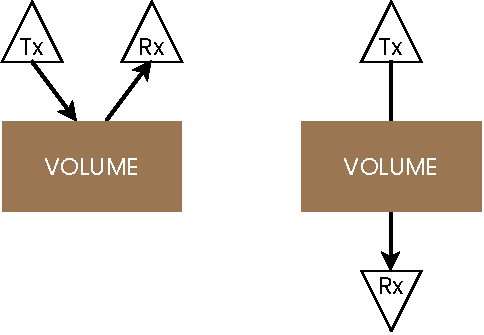
\includegraphics[width=0.8\textwidth]{images/theoretical/GPR20_surveying.pdf}
    \caption{GPR measurement types. The left side depicts the reflection type while the right depicts the transillumination.}
    \label{fig:surveying}
\end{figure}

The foundations of GPR lie in the electromagnetic (EM) theory, which uses the Maxwell's equations to mathematically describe the physics of EM fields. Constitutive relationships are used to quantify material properties. Maxwell equations are presented in equations (\ref{eq:max_1}) to (\ref{eq:max_4}) where $\bar{E}$ is the electric field strength vector ($V/m$); $q$ is the electric charge density ($C/m^{3}$); $\bar{B}$ is the magnetic flux density vector ($T$); $\bar{J}$ is the electric current density vector ($A/m^{2}$); $\bar{D}$ is the electric displacement vector ($C/m^{2}$); $t$ is time ($s$); and $\bar{H}$ is the magnetic field density ($A/m$).
\begin{align}
    \bar{\nabla} \times \bar{E} &= - \frac{\partial \bar{B}}{\partial t} \label{eq:max_1} \\
    \bar{\nabla} \times \bar{H} &= \bar{J} + \frac{\partial \bar{D}}{\partial t} \label{eq:max_2} \\
    \bar{\nabla} \cdot \bar{D} &= q \label{eq:max_3} \\
    \bar{\nabla} \cdot \bar{B} &= 0 \label{eq:max_4}
\end{align}
The first equation (\ref{eq:max_1}) is known as the Maxwell-Faraday equation, and describes the relationship between an electric field and a magnetic field. The second equation (\ref{eq:max_2}) is known as the Ampère-Maxwell equation, and describes how magnetic fields can induct electrical fields under certain conditions. The third equation (\ref{eq:max_3}) is known as the Gauss's law and describes how electric fields relate to electrical charges. Finally, the fourth law (\ref{eq:max_4}) is known as the Gauss's law for magnetism and states that magnetic fields must be the product of a magnetic dipole thus ruling out magnetic monopoles.

Constitutive equations are presented in equations (\ref{eq:const_1}) to (\ref{eq:const_3}) where $\tilde{\sigma}$ is the electrical conductivity; $\tilde{\epsilon}$ is the dielectric permittivity; and $\tilde{\mu}$ is the magnetic conductivity. The first constitutive equation (\ref{eq:const_1}) presents how electric current is created, and resisted, in a material when an electric field is applied. The second equation (\ref{eq:const_2}) tells that energy storage is creates when a material is subject to an electrical field. The energy storage is mathematically defined as the electrical displacement vector. Finally, the third equation (\ref{eq:const_3}) indicates how a material responds to a magnetic field. 
\begin{align}
    \bar{J} &= \tilde{\sigma} \bar{E} \label{eq:const_1} \\
    \bar{D} &= \tilde{\epsilon} \bar{E} \label{eq:const_2} \\
    \bar{B} &= \tilde{\mu} \bar{H} \label{eq:const_3}
\end{align}
Both the Maxwell equations and the constitutive equations describe how EM waves travel through different materials. As stated previously, GPR is used in low-loss materials. Electrical losses depend on the electrical conductivity ($\tilde{\sigma}$) of the material. The maximum depth of a GPR sampling depends on the electrical conductivity of a material. A high conductivity will imply that EM waves would travel deeper since less energy is dissipated (low-loss). On the other hand, a low conductivity material will dissipate more energy (high-loss) so EM waves would not travel as deeply. 

In practice, soil is not homogeneous thus EM waves interact with different materials with different EM characteristics. Both low-loss and high-loss materials can be present in the soil under different composition ratios. Soil can be composed of soil grains, air, water and objects such as rocks. However, evidence has show that water response to EM waves is one of the most dominant behaviors when GPR data is acquired.

Radio waves are electromagnetic (EM) waves that can be described with a wave equation. By examining the wave equation it is possible to further identify wave characteristics under specific materials. It is possible to derive the wave equation of EM fields from the Maxwell equations and the constitutive equations. In order to derive the wave equation, the first step is to include the constitutive equations into the Ampère-Maxwell equation to use the $\bar{B}$ and $\bar{E}$ vectors. The result of the process is presented in equation (\ref{eq:max_2_raw}).
\begin{align}
    \bar{\nabla} \times \bar{H} &= \bar{J} + \frac{\partial \bar{D}}{\partial t} & \bar{H} &= \tilde{\mu}^{-1} \bar{B} & \bar{J} &= \tilde{\sigma} \bar{E} & \bar{D} &= \tilde{\epsilon} \bar{E} \nonumber \\
    \bar{\nabla} \times (\tilde{\mu}^{-1} \bar{B}) &= \tilde{\sigma} \bar{E} + \frac{\partial (\tilde{\epsilon} \bar{E})}{\partial t} \nonumber \\
    \tilde{\mu}^{-1} (\bar{\nabla} \times \bar{B}) &= \tilde{\sigma} \bar{E} + \tilde{\epsilon} \frac{\partial \bar{E}}{\partial t} \nonumber \\
    \bar{\nabla} \times \bar{B} &= \tilde{\mu} \tilde{\sigma} \bar{E} + \tilde{\mu} \tilde{\epsilon} \frac{\partial \bar{E}}{\partial t} \label{eq:max_2_raw}
\end{align}
The second step is to take the curl of the curl of the electric field strength vector ($\bar{E}$) which corresponds to taking the curl of the Maxwell-Faraday equation. Once vector calculus identities are applied, it is possible to incorporate the Ampère-Maxwell equation in the form presented on equation (\ref{eq:max_2_raw}). The result of the process is presented in equation (\ref{eq:wave_eq}). This equation corresponds to a wave equation in which three terms can be identified with the second ($ \tilde{\mu} \tilde{\sigma} \frac{\partial \bar{E}}{\partial t}$) being related to energy dissipation and the third ($\tilde{\mu} \tilde{\epsilon} \frac{\partial^{2} \bar{E}}{\partial t^{2}}$) being related to energy storage. The GPR is useful in situations where the energy dissipation is considerable lower than the energy storage.
\begin{align}
    \bar{\nabla} \times (\bar{\nabla} \times \bar{E}) &= \bar{\nabla} \times \left( - \frac{\partial \bar{B}}{\partial t} \right) \nonumber \\
    \bar{\nabla} \times \bar{\nabla} \times \bar{E} &= - \frac{\partial}{\partial t} (\bar{\nabla} \times \bar{B}) \nonumber \\
    \bar{\nabla} \times \bar{\nabla} \times \bar{E} &= - \frac{\partial}{\partial t} (\tilde{\mu} \tilde{\sigma} \bar{E} + \tilde{\mu} \tilde{\epsilon} \frac{\partial \bar{E}}{\partial t}) \nonumber \\
    \bar{\nabla} \times \bar{\nabla} \times \bar{E} &= - \tilde{\mu} \tilde{\sigma} \frac{\partial \bar{E}}{\partial t} + \tilde{\mu} \tilde{\epsilon} \frac{\partial^{2} \bar{E}}{\partial t^{2}} \nonumber \\
     \bar{\nabla} \times \bar{\nabla} \times \bar{E} + \tilde{\mu} \tilde{\sigma} \frac{\partial \bar{E}}{\partial t} + \tilde{\mu} \tilde{\epsilon} \frac{\partial^{2} \bar{E}}{\partial t^{2}} &= 0 \label{eq:wave_eq}
\end{align}
Solving the wave equation is non-trivial and requires to make assumptions. Assumptions include using scalar values for the dielectric permittivity ($\tilde{\epsilon} \approx \epsilon$), electric conductivity ($\tilde{\sigma} \approx \sigma$) and magnetic permeability ($\tilde{\mu} \approx \mu$). The process of solving the wave equation is not presented because of its length and complexity. Electric ($E$) and magnetic ($B$) fields are found to be orthogonal when solving the wave equation. There is a third vector that is orthogonal to both the electric and magnetic fields and represents the spatial direction of the field movement. The field movement direction is denoted with $\hat{K}$. Solving the wave equation defines two values that are relevant for the GPR surveying process: wave velocity ($v$) and wave attenuation ($\alpha$). The values of both $v$ and $\alpha$ are defined in equations (\ref{eq:velocity}) and (\ref{eq:attenuation}).
\begin{align}
    v &= \frac{1}{\sqrt{\epsilon \mu}} \label{eq:velocity} \\
    \alpha &= \frac{1}{2} \sigma \sqrt{\frac{\mu}{\epsilon}} \label{eq:attenuation}
\end{align}
Considering that EM waves exhibit an oscillation nature, frequency ($f$) is key to understand the materials' response. Two major behaviors are generalized when characterizing the frequency-response of materials: a diffusive field behaviour and an independent behaviour. The diffusive field behaviour occurs at low frequencies and is not used for GPR sampling. On the other hand, independent behavior occurs at high-frequencies and is used for GPR. A transition frequency ($f_{t}$) can be determined to establish the GPR survey in the right conditions. The transition frequency of a simple material can be calculated with equation (\ref{eq:trans_freq}).
\begin{equation}
    f_{t} = \frac{\sigma}{2\pi \epsilon}
    \label{eq:trans_freq}
\end{equation}
Values of velocity ($v$), attenuation ($\alpha$) and impedance ($Z$) are key wave properties. Both the velocity and attenuation can be further expressed in terms of constants such as light speed ($c$), dielectric constant ($\kappa$) and impedance of free space ($Z_{0}$). The dielectric constant refers to the ratio between a material's dielectric permittivity and the vacuum dielectric permittivity ($\kappa = \frac{\epsilon}{\epsilon_{0}}$). Light speed can also be defined in terms of both the vacuum's dielectric permittivity ($\epsilon_{0}$) and magnetic permeability ($\mu_{0}$) with $c=\frac{1}{\sqrt{\epsilon_{0}\mu_{0}}}$. Impedance of free space is defined as $Z_{0} = \sqrt{\frac{\mu_{0}}{\epsilon_{0}}}$. Values of velocity ($v$), attenuation ($\alpha$) and impedance ($Z$) are defined in equations (\ref{eq:vel}) to (\ref{eq:imp}).
\begin{align}
    v &= \frac{c}{\sqrt{\kappa}} \label{eq:vel} \\ 
    \alpha &= Z_{0} \frac{\sigma}{2\sqrt{\kappa}} \label{eq:att} \\
    Z &= \frac{Z_{0}}{\sqrt{\kappa}} \label{eq:imp}
\end{align}
Material interfaces play a major role in GPR sampling. Characterizing how waves travel after reaching interfaces is crucial for GPR analysis. Two possibilities can arise at an interface depending on the source: either the source is above the interface or in the interface. It is relevant to characterize how waves travel with the source at the interface since GPR data is acquired with the antennae (source) located near the ground. Waves can be either reflected of refracted at an interface. Reflection and refraction of waves operate according to Snell's law and Fresnel coefficients with critical situations defining the boundaries.

Four signal types can be identified in a GPR sample: a direct air wave, a direct ground wave, a critically refracted ground wave and a reflected wave. The direct air wave are the signals that travel from the transmitter to the receiver directly i.e. through the air that separates them. Direct ground waves correspond to signals that enter the ground in such a way that they travel through the interface and then back to the receiver. Critically refracted waves are signals that reach a further interface, get refracted only to be refracted back in the air/ground interface towards the receiver. Reflected waves are signals that get reflected in a further interface but travel directly to the receiver. Figure \ref{fig:waves} illustrates how these signals behave. As signals use different paths, time-delays and amplitude differences for each signal are expected. These time-delays and amplitudes are what is effectively being measured by the GPR.

\begin{figure}
    \centering
    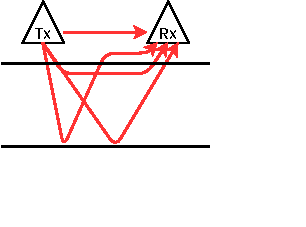
\includegraphics[width=0.7\textwidth, trim = 0cm 1cm 2cm 0cm, clip]{images/theoretical/GPR20_surveying_waves.pdf}
    \caption{Signal types for a GPR sampling.}
    \label{fig:waves}
\end{figure}

GPR data is acquired through reflection or transillumination. The GPR-20 robot uses the reflection thus transillumination will not be discussed. Reflection uses a transmitter and a receiver in a fixed geometry to acquire data. Multiple transmitter and receivers can be used depending on the application of the GPR. The antennae geometry are defined by a separation and an orientation. This geometry is moved along an axis with measurements on predefined intervals. The measurements consists of acquiring data that will present different time-delays and amplitudes that are the result of variations in the $v$, $\alpha$ and $Z$ wave parameters for the underground materials.

\section{GPR-20 Radar Implementation}
The Ground Penetrating Radar (GPR) technique is implemented in the GPR-20 robot using a Vector Network Analyzer (VNA) and two antennae. The VNA and the antennae are attached to a physical structure that is known as the positioner. The positioner includes two motors to rotate the antennae in order to acquire data with different orientations. The positioner is shown in figure \ref{fig:positioner} where the antennae and the VNA case can be identified. The antennae are located in the bottom of the structure while the VNA is located at the top of it. The antennae are separated by a distance of 310 millimeters. The antennae separation is enough for the antennae to operate in two orientations and to rotate to their position without colliding. Distance from the antennae to the ground can be customized depending on the environment. The distance between the ground and the antennae support is measured using an infrared sensor. The positioner is designed to move within a sampling area in two perpendicular directions, thus enabling a two-dimensional movement.

\begin{figure}[h]
    \centering
    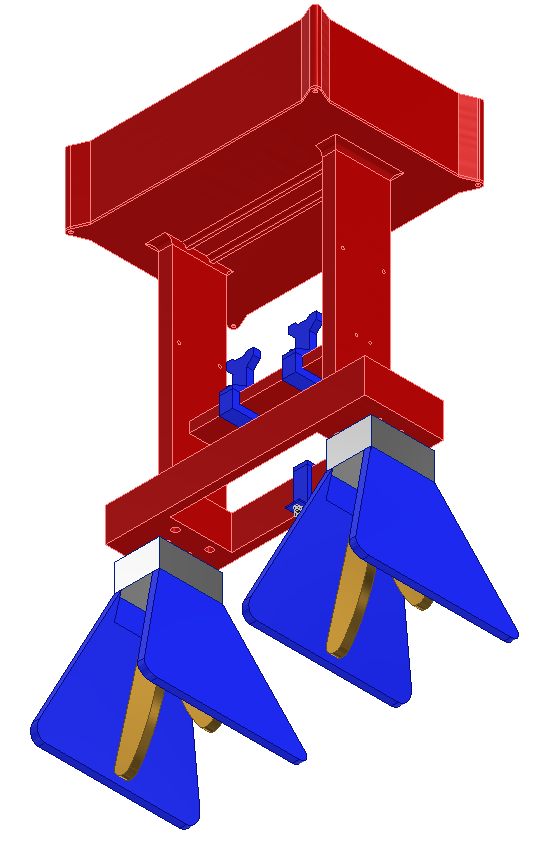
\includegraphics[width=0.4\textwidth]{images/implementation/positioner_a.png}
    \caption{Positioner of the GPR-20 robot.}
    \label{fig:positioner}
\end{figure}

The GPR-20 robot uses an Anritsu MS2026C VNA (\href{https://dl.cdn-anritsu.com/en-us/test-measurement/files/Brochures-Datasheets-Catalogs/datasheet/11410-00548AM.pdf}{datasheet}) and two Aaronia PowerLOG 70180 antennae (\href{https://downloads.aaronia.com/datasheets/antennas/PowerLOG/Aaronia_PowerLOG_Horn_Antennas.pdf##}{datahseet}) to acquire GPR data. The VNA is used to send pulses to the transmitter antenna and measure the response from the receiver signal. Data is acquired in the frequency-domain and is exported from the VNA using the VXI-11 protocol to processing and storage devices. Table \ref{tab:vna_specs} presents the specifications for the MS2026C VNA device. Table \ref{tab:antenna_specs} presents the Aaronia PowerLOG 70180 antenna specifications.

\begin{table}[h]
    \centering
    \begin{tabular}{|l|l|}
        \hline \textbf{Specification} & \textbf{Value} \\ \hline
        Bandwidth & 5kHz to 6GHz \\ \hline
        Ports & Two (2) \\ \hline
        Accuracy & 12-term \\ \hline
        Data Points & Up to 4001 \\ \hline
        Sweep Speed & $350 \mu s$ per point \\ \hline
        Data Interfaces & USB/Ethernet \\ \hline
        Weight & 4.5/4.9 kg \\ \hline
        Datasheet & \href{https://dl.cdn-anritsu.com/en-us/test-measurement/files/Brochures-Datasheets-Catalogs/datasheet/11410-00548AM.pdf}{Link} \\ \hline
    \end{tabular}
    \caption{Specifications for the Anritsu MS2026C VNA.}
    \label{tab:vna_specs}
\end{table}

\begin{table}[h]
    \centering
    \begin{tabular}{|l|l|}
        \hline \textbf{Specifications} & \textbf{Value} \\ \hline
        Dimensions & 235$\times$252$\times$175 mm \\ \hline
        Weight & 1400 g \\ \hline
        Design & Dual-ridged Horn \\ \hline
        Gain & 2 - 17 dBi \\ \hline
        Frequency Range & 700Mhz - 18GHz \\ \hline
        Nominal Impedance & 50 Ohms \\ \hline
        Datasheet & \href{https://downloads.aaronia.com/datasheets/antennas/PowerLOG/Aaronia_PowerLOG_Horn_Antennas.pdf##}{Link} \\ \hline
    \end{tabular}
    \caption{Aaronia PowerLOG 70180 antenna specifications.}
    \label{tab:antenna_specs}
\end{table}


\section{Field Data-Acquisition Process}
The process of data-acquisition will be presented in this section. The process of data-acquisition consists of the specific procedures that must take place in the GPR-20 robot to acquire data from a sampling area. Pre-acquisition and post-acquisition procedures will also be discussed to give the reader a general overview of what it takes to acquire data. 

The robot and the equipment must be setup before the data acquisition process takes place. This setup consists of configuring the network and power connections. Network connections are configured using a network switch and a Local Area Network (LAN). The robot, VNA, and an additional personal computer must be linked to the network via Ethernet cables. The LAN will assign an IP address to each device that will be used during the data acquisition process. Power connections consists of connecting the devices into a reliable power supply. The connections are made using standard power plugs to an AC power outlet. Four (4) devices must be connected: the personal computer, the VNA, the robot itself, and the network switch. Table \ref{tab:net_power_conn} summarizes the power and network setup process.

\begin{singlespace}
    \begin{xltabular}{\textwidth}{|c|X|}
    
        \endhead
        
        \caption{Network and power connections for the GPR-20 robot.} \label{tab:net_power_conn}
        \endlastfoot
        
        \multicolumn{2}{|c|}{\textit{Continues on next page.}}
        \endfoot
        
        \hline \multicolumn{2}{|c|}{\textbf{Network Setup}} \\ \hline
        $\square$ & Connect the personal computer to the network switch using an Ethernet cable. \\ \hline
        $\square$ & Connect the VNA to the network switch using an Ethernet cable. \\ \hline
        $\square$ & Connect the GPR-20 robot to the network switch using an Ethernet cable. \\ \hline
        \multicolumn{2}{|c|}{\textbf{Power Setup}} \\ \hline
        $\square$ & Connect the network switch to the AC power supply \\ \hline
        $\square$ & Connect the personal computer to the AC power supply \\ \hline
        $\square$ & Connect the VNA to the AC power supply \\ \hline
        $\square$ & Connect the GPR-20 robot to the AC power supply \\ \hline
    \end{xltabular}
\end{singlespace}

Installing and configuring the Robot Operating System (ROS, \href{https://ros.org/}{webpage}) is required in order to use the GPR-20 robot. ROS must be installed and configured in both the personal computer and the GPR-20 robot on-board computer. Both devices are assumed to be using a desktop Linux Ubuntu distribution (\href{https://ubuntu.com/}{webpage}) as their Operating System (OS). The recommended OS distribution is Ubuntu 18.04 although Ubuntu 20.04 will also work. Each Ubuntu version (18.04 or 20.04) has its own corresponding ROS version. ROS \textit{Melodic} is intended to be used with Ubuntu 18.04 while ROS \textit{Noetic} is intended to Ubuntu 20.04. Installation and configuration of ROS is presented in the official documentation (\href{http://wiki.ros.org/melodic/Installation/Ubuntu}{ROS \textit{Melodic}}, \href{http://wiki.ros.org/noetic/Installation/Ubuntu}{ROS \textit{Noetic}}).

ROS relies on packages to incorporate software into the applications. By using these packages, in which the different utilities are implemented, different functionalities can be used. The GPR-20 robot has six (6) ROS packages that implement all the required functionalities. Depending on its computational resource usage, software packages are intended to be used in either the personal computer or the on-board computer. The utilities reserved for the on-board computer usage are the \texttt{Axis Driver}, \texttt{Height Sensor}, \texttt{Main Control} and \texttt{User Interface}. On the other hand, the \texttt{VNA Acquisition} and \texttt{VNA Processing} utilities are intended to be used in the personal computer. ROS only requires packages to be placed in a workspace in order to use them. However, some packages rely on third-party libraries that must be installed in order to execute certain functionalities. Table \ref{tab:package_installation} presents the procedure for adding a package, identifying the required third-party libraries, and install them. Furthermore, table \ref{tab:software_repos} presents the software utilities with the links to their respective repositories.

\begin{singlespace}
    \begin{xltabular}{\textwidth}{|c|X|}
    
        \caption{Procedure for adding a package into a host computer.} \label{tab:package_installation}
        \endlastfoot
    
        \hline \multicolumn{2}{|c|}{\textbf{Workspace Configuration}} \\ \hline
        $\square$ & Create a workspace in the host computer. The workspace consists of a parent directory (\texttt{<name>\_ws}) with a sub-folder named \texttt{src}. If a workspace has been already created, use the existing one. \\ \hline
        $\square$ & Place the package into the \texttt{src} sub-folder of the workspace. \\ \hline
        $\square$ & Execute the \texttt{catkin\_make} command on the workspace directory. Wait for the command for exit without errors. \\ \hline
        $\square$ & Source the workspace by executing \texttt{source devel/setup.bash}. \\ \hline
        \multicolumn{2}{|c|}{\textbf{Third-party Libraries Installation}} \\ \hline
        $\square$ & Identify the third-party libraries requirements in the software packages repositories. The required libraries and their considerations are presented in the repository read-me file. \\ \hline
        $\square$ & Install the third-party libraries and ensure that they are correctly working in the host computer. \\ \hline
    \end{xltabular}
\end{singlespace}

\begin{singlespace}
    \begin{xltabular}{\textwidth}{|l|X|}
    
        \hline \textbf{Repository} & \textbf{Link} \\ \hline
        \endhead
        
        \caption{Software packages with their respective repositories.} \label{tab:software_repos}
        \endlastfoot
        
        Axis Driver & \url{https://github.com/gdh-uniandes/gpr20_axis_driver} \\ \hline
        Height Sensor & \url{https://github.com/gdh-uniandes/gpr20_height_sensor} \\ \hline
        VNA Acquisition & \url{https://github.com/gdh-uniandes/gpr20_vna_acquisition} \\ \hline
        VNA Processing & \url{https://github.com/gdh-uniandes/gpr20_vna_processing} \\ \hline
        Main Control & \url{https://github.com/gdh-uniandes/gpr20_main_control} \\ \hline
        User Interface & \url{https://github.com/gdh-uniandes/gpr20_user_interface} \\ \hline
    \end{xltabular}
\end{singlespace}

Although the six (6) packages are needed for the data acquisition, some of them are directly linked to the process itself. The \texttt{VNA Acquisition}, \texttt{VNA Processing}, and \texttt{Main Control}. Configuration of these software packages is done via the user interface. Ten (10) parameters define the data acquisition process. Six (6) parameters are used to define the physical movement of the radar within the sampling area. These parameters correspond to the start coordinate for the X and Y axes, the stop coordinate for the X and Y axes, and the number of points to be sampled on each axes. The remaining four (4) parameters correspond to the start and stop frequencies for the VNA, the sampled frequency points and the VNA IP address.

Before starting the data-acquisition process, the VNA must be calibrated. The calibration ensures that data will be acquired with the best quality. The calibration process depends on both the used VNA device and the used, or available calibration methodology. Since the VNA can be calibrated prior to the data-acquisition, it is required for the device to heat up until reaching its operating temperature. Some devices include a feedback capability in which the device itself can evaluate its calibration status. The calibration status for a VNA device used in the GPR data acquisition must be as high as possible. The VNA calibration will be relevant and crucial for the whole data acquisition process. 

Once the device is calibrated, antennae are connected to the VNA ports. The antennae might use adapters which must be compensated in the calibration. The compensation can be executed in the calibration although this depends on the specific calibration methodology that is being used. Once antennae are connected, they must be physically arranged in such a way that they are parallel to each other. Once antennae are connected to the VNA and physically located in their initial position, it is possible to configure the surveying process.

The user is now able to power the robot and define the survey parameters in the user interface. The user will input the parameters in the graphical interface and command the robot to start the survey. The survey process will move the positioner to its initial coordinate after executing the homing routine. From then, the positioner will continue to move along the coordinate values in the grid pattern. Each time the positioner reaches a sampling coordinate, data will be acquired from two different polarizations. This is achieved by precisely rotating the antennae ninety degrees ($90^{\circ}$) from their initial position. The movement of the axes motors is executed through the \texttt{Axis Driver} utility with the target coordinates being sent from the \texttt{Main Control}. The storage process is executed in parallel to the data acquisition in order to reduce memory consumption and keep it safely from power shortages.

Data is stored in the JSON format. This format allows to store different features of the data besides from the VNA response. The format stores the coordinates where the data value was acquired (X and Y linear coordinates and Z rotational coordinate). These coordinates will be used in the data processing stage. Height of the antennae is also stored in the JSON file. A time stamp and two unique identifiers are also stored in these files. The time stamp is used for data record purposes. On the other hand, one identifier will be assigned to the survey as a whole while the other one is assigned to each data file. Finally, the VNA data itself will be stored in the JSON file. Listing \ref{lst:json_file} presents an example of the used JSON file.

\begin{singlespace}
    \begin{lstlisting}[
            caption={JSON example file for storing each measurement.},
            label={lst:json_file}
        ]
        {
            ``x_coord": <X axis coordinate>,
            ``y_coord": <Y axis coordinate>,
            ``z_coord": <Z rotation coordinate>,
            ``antennae_height": <Antennae height>,
            ``timestamp": <Time stamp>,
            ``survey_id": <Survey unique identifier>,
            ``sample_id": <Sample unique identifier>,
            ``data": [
                [
                    ``freq_value": <Frequency value>,
                    ``param_value": <S21 parameter value>
                ],
                ...,
                [
                    ``freq_value": <Frequency value>,
                    ``param_value": <S21 parameter value>
                ]
            ]
        }
    \end{lstlisting}
\end{singlespace}

Data can be processed once the data acquisition process finishes. The data processing can start with the process of generating A, B and C-scans to visualize the results. An A-Scan is the time-domain data that is sampled from a specific coordinate and polarization. The amplitude of the A-Scan at a given time represents the reflections of a ground feature at an specific depth. A B-Scan represents the results from data acquired along a single linear axis. The B-Scan is an image-like array of data in which the results of multiple A-Scans are visualized. B-Scan allow the visualization of underground features that may not be detected using A-Scans. Finally, C-Scans provide a three-dimensional data representation of the whole sampled area by adding multiple B-Scans.

Data processing does not stop with data visualization. Data-cleaning and feature-enhancing processing can be executed over data to improve its quality and results. Data-cleaning can be performed using a broad range of algorithms with different complexities. A similar situation arise with feature-enhancing processing. Data can be used to feed different models and algorithms to solve the landmine detection problem. However, processing of data and its usage is currently out of the scope for the GPR-20 data acquisition mechanisms.

\section{Future Work}
GPR-20 is a tool that might enable the acquisition on quality Ground Penetrating Radar (GPR) data. Extensions can be implemented to enhance the robot capabilities and to ease the procedure of data-acquisition and data-processing. Extensions are mainly focused on the landmine detection problem yet they might apply to other GPR-related problems. Extensions include adding processing stages or generating A, B and C scans during the data-acquisition, and use the data to train models for landmine detection.

The first extension that can be implemented in the data acquisition and processing pipeline is a cleaning stage. This cleaning stage will attempt to eliminate persistent yet non-relevant features from the data. Direct air waves and direct ground waves could be eliminated to increase the relevance of other data features. Applying a time gain to the sample signal can be also incorporated into the processing pipeline. It must be noted that raw data will be always stored since it allows for multiple processing techniques to be tested.

Generating A, B and C scans during the surveying process can be also implemented in the GPR-20 robot. Providing these visualization elements in the graphical interface could improve the user experience of the robot user. Generating both the A and B scans is not a complex task since data is available as soon as it is acquired. A-Scans only require converting data from the frequency-domain to time-domain using an inverse Fourier transform. B-Scans can be created dynamically as data is being acquired for a given linear axis. However, C-Scans require extensive computer processing to be generated. C-Scan may be the most challenging visualization element to be generated during data acquisition.

Landmine detection can be executed parallel to data acquisition. Different models and algorithms could be used to tell whether an specific sample has a landmine or not. The sample can consist of either data acquired from a single coordinate or the whole set of data from a sampled area. There is no doubt that different models and algorithms must be tested in order to define which data will be used as the input of a landmine detection system. On the other hand, a large amount of data, under different scenarios, must be acquired in order to train and test the different models and/or algorithms. 


\end{document}
